\tikzset{every picture/.style={line width=0.75pt}} %set default line width to 0.75pt        

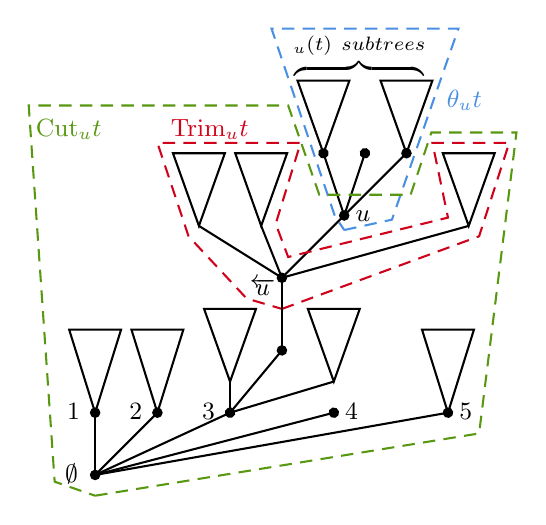
\begin{tikzpicture}[x=0.75pt,y=0.75pt,yscale=1,xscale=1]
%uncomment if require: \path (0,325); %set diagram left start at 0, and has height of 325

%Straight Lines [id:da8807462266894251] 
\draw    (160,120) -- (120,145) ;
%Straight Lines [id:da11953613879967617] 
\draw    (70,25) -- (185,55) ;
\draw [shift={(185,55)}, rotate = 14.62] [color={rgb, 255:red, 0; green, 0; blue, 0 }  ][fill={rgb, 255:red, 0; green, 0; blue, 0 }  ][line width=0.75]      (0, 0) circle [x radius= 2.01, y radius= 2.01]   ;
%Straight Lines [id:da9015232480401707] 
\draw    (70,25) -- (70,55) ;
\draw [shift={(70,55)}, rotate = 90] [color={rgb, 255:red, 0; green, 0; blue, 0 }  ][fill={rgb, 255:red, 0; green, 0; blue, 0 }  ][line width=0.75]      (0, 0) circle [x radius= 2.01, y radius= 2.01]   ;
\draw [shift={(70,25)}, rotate = 90] [color={rgb, 255:red, 0; green, 0; blue, 0 }  ][fill={rgb, 255:red, 0; green, 0; blue, 0 }  ][line width=0.75]      (0, 0) circle [x radius= 2.01, y radius= 2.01]   ;
%Straight Lines [id:da5129436960048647] 
\draw    (70,25) -- (100,55) ;
\draw [shift={(100,55)}, rotate = 45] [color={rgb, 255:red, 0; green, 0; blue, 0 }  ][fill={rgb, 255:red, 0; green, 0; blue, 0 }  ][line width=0.75]      (0, 0) circle [x radius= 2.01, y radius= 2.01]   ;
%Straight Lines [id:da772575048942949] 
\draw    (135,55) -- (160,85) ;
\draw [shift={(160,85)}, rotate = 50.19] [color={rgb, 255:red, 0; green, 0; blue, 0 }  ][fill={rgb, 255:red, 0; green, 0; blue, 0 }  ][line width=0.75]      (0, 0) circle [x radius= 2.01, y radius= 2.01]   ;
%Straight Lines [id:da6325690221327983] 
\draw    (70,25) -- (240,55) ;
\draw [shift={(240,55)}, rotate = 10.01] [color={rgb, 255:red, 0; green, 0; blue, 0 }  ][fill={rgb, 255:red, 0; green, 0; blue, 0 }  ][line width=0.75]      (0, 0) circle [x radius= 2.01, y radius= 2.01]   ;
%Straight Lines [id:da3473141510675146] 
\draw    (135,55) -- (135,70) ;
%Straight Lines [id:da16274072806702156] 
\draw    (190,150) -- (200,180) ;
\draw [shift={(200,180)}, rotate = 71.57] [color={rgb, 255:red, 0; green, 0; blue, 0 }  ][fill={rgb, 255:red, 0; green, 0; blue, 0 }  ][line width=0.75]      (0, 0) circle [x radius= 2.01, y radius= 2.01]   ;
%Straight Lines [id:da5025794992551161] 
\draw    (135,55) -- (185,70) ;
%Straight Lines [id:da7415577835604696] 
\draw    (190,150) -- (180,180) ;
\draw [shift={(180,180)}, rotate = 108.43] [color={rgb, 255:red, 0; green, 0; blue, 0 }  ][fill={rgb, 255:red, 0; green, 0; blue, 0 }  ][line width=0.75]      (0, 0) circle [x radius= 2.01, y radius= 2.01]   ;
%Straight Lines [id:da5320526201995357] 
\draw    (190,150) -- (220,180) ;
\draw [shift={(220,180)}, rotate = 45] [color={rgb, 255:red, 0; green, 0; blue, 0 }  ][fill={rgb, 255:red, 0; green, 0; blue, 0 }  ][line width=0.75]      (0, 0) circle [x radius= 2.01, y radius= 2.01]   ;
%Straight Lines [id:da3923916194254533] 
\draw    (160,120) -- (150,145) ;
%Straight Lines [id:da7281718161332553] 
\draw    (160,120) -- (190,150) ;
\draw [shift={(190,150)}, rotate = 45] [color={rgb, 255:red, 0; green, 0; blue, 0 }  ][fill={rgb, 255:red, 0; green, 0; blue, 0 }  ][line width=0.75]      (0, 0) circle [x radius= 2.01, y radius= 2.01]   ;
%Shape: Triangle [id:dp061408321195388194] 
\draw  [line width=0.75]  (70,55) -- (82.5,95) -- (57.5,95) -- cycle ;
%Shape: Triangle [id:dp18467641596455997] 
\draw  [line width=0.75]  (100,55) -- (112.5,95) -- (87.5,95) -- cycle ;
%Straight Lines [id:da4332998583593296] 
\draw    (70,25) -- (135,55) ;
\draw [shift={(135,55)}, rotate = 24.78] [color={rgb, 255:red, 0; green, 0; blue, 0 }  ][fill={rgb, 255:red, 0; green, 0; blue, 0 }  ][line width=0.75]      (0, 0) circle [x radius= 2.01, y radius= 2.01]   ;
%Shape: Triangle [id:dp7432900095669139] 
\draw  [line width=0.75]  (135,70) -- (147.5,105) -- (122.5,105) -- cycle ;
%Straight Lines [id:da7580937057804584] 
\draw    (160,120) -- (250,145) ;
%Shape: Triangle [id:dp31826184866501805] 
\draw  [line width=0.75]  (185,70) -- (197.5,105) -- (172.5,105) -- cycle ;
%Shape: Triangle [id:dp11283996969265198] 
\draw  [line width=0.75]  (240,55) -- (252.5,95) -- (227.5,95) -- cycle ;
%Shape: Triangle [id:dp7050388122593998] 
\draw  [line width=0.75]  (120,145) -- (132.5,180) -- (107.5,180) -- cycle ;
%Shape: Triangle [id:dp45624316372209406] 
\draw  [line width=0.75]  (150,145) -- (162.5,180) -- (137.5,180) -- cycle ;
%Shape: Triangle [id:dp8097356363166169] 
\draw  [line width=0.75]  (250,145) -- (262.5,180) -- (237.5,180) -- cycle ;
%Shape: Triangle [id:dp5118714347287557] 
\draw  [line width=0.75]  (180,180) -- (192.5,215) -- (167.5,215) -- cycle ;
%Shape: Triangle [id:dp9899984672182544] 
\draw  [line width=0.75]  (220,180) -- (232.5,215) -- (207.5,215) -- cycle ;
%Shape: Polygon [id:ds08310512731475861] 
\draw  [color={rgb, 255:red, 74; green, 144; blue, 226 }  ,draw opacity=1 ][dash pattern={on 4.5pt off 3pt}] (190,143) -- (213,148) -- (245,240) -- (155,240) -- (185.5,149.75) -- cycle ;
%Shape: Polygon [id:ds8180957148225936] 
\draw  [color={rgb, 255:red, 208; green, 2; blue, 27 }  ,draw opacity=1 ][dash pattern={on 4.5pt off 3pt}] (160,105) -- (255,140) -- (269.5,185) -- (232.5,185) -- (240,149) -- (163,130) -- (157,146) -- (169,185) -- (100,185) -- (115,140) -- (143,110) -- cycle ;
%Shape: Polygon [id:ds27551258730036354] 
\draw  [color={rgb, 255:red, 88; green, 152; blue, 17 }  ,draw opacity=1 ][dash pattern={on 4.5pt off 3pt}] (70,15) -- (255,45) -- (273,190) -- (232,190) -- (222,160) -- (178,160) -- (163,203) -- (38,203) -- (50.5,21.75) -- cycle ;
%Straight Lines [id:da4474134185419224] 
\draw    (160,85) -- (160,120) ;
\draw [shift={(160,120)}, rotate = 90] [color={rgb, 255:red, 0; green, 0; blue, 0 }  ][fill={rgb, 255:red, 0; green, 0; blue, 0 }  ][line width=0.75]      (0, 0) circle [x radius= 2.01, y radius= 2.01]   ;

% Text Node
\draw (54,19.4) node [anchor=south west][inner sep=0.75pt]  [font=\small,color={rgb, 255:red, 0; green, 0; blue, 0 }  ,opacity=1 ]  {$\emptyset $};
% Text Node
\draw (55,50.4) node [anchor=south west][inner sep=0.75pt]  [font=\small,color={rgb, 255:red, 0; green, 0; blue, 0 }  ,opacity=1 ]  {$1$};
% Text Node
\draw (189,50.4) node [anchor=south west][inner sep=0.75pt]  [font=\small,color={rgb, 255:red, 0; green, 0; blue, 0 }  ,opacity=1 ]  {$4$};
% Text Node
\draw (244,50) node [anchor=south west][inner sep=0.75pt]  [font=\small,color={rgb, 255:red, 0; green, 0; blue, 0 }  ,opacity=1 ] [align=left] {$\displaystyle 5$};
% Text Node
\draw (85,50.4) node [anchor=south west][inner sep=0.75pt]  [font=\small,color={rgb, 255:red, 0; green, 0; blue, 0 }  ,opacity=1 ]  {$2$};
% Text Node
\draw (120,50.4) node [anchor=south west][inner sep=0.75pt]  [font=\small,color={rgb, 255:red, 0; green, 0; blue, 0 }  ,opacity=1 ]  {$3$};
% Text Node
\draw (194,145.4) node [anchor=south west][inner sep=0.75pt]  [font=\small,color={rgb, 255:red, 0; green, 0; blue, 0 }  ,opacity=1 ]  {$u$};
% Text Node
\draw (143,110) node [anchor=south west][inner sep=0.75pt]  [font=\small,color={rgb, 255:red, 0; green, 0; blue, 0 }  ,opacity=1 ]  {$\overleftarrow{u}$};
% Text Node
\draw (238,199) node [anchor=south west][inner sep=0.75pt]  [font=\small,color={rgb, 255:red, 74; green, 144; blue, 226 }  ,opacity=1 ] [align=left] {$\displaystyle \theta _{u} t$};
% Text Node
\draw (164,214.4) node [anchor=south west][inner sep=0.75pt]  [font=\normalsize]  {$\overbrace{\ \ \ \ \ \ \ \ \ \ \ \ \ \ }^{\rk_{u}(t) \ \text{subtrees}}$};
% Text Node
\draw (105,185) node [anchor=south west][inner sep=0.75pt]  [font=\small,color={rgb, 255:red, 208; green, 2; blue, 27 }  ,opacity=1 ] [align=left] {$\displaystyle \mathrm{Trim}_{u} t$};
% Text Node
\draw (40,185) node [anchor=south west][inner sep=0.75pt]  [font=\small,color={rgb, 255:red, 88; green, 152; blue, 17 }  ,opacity=1 ] [align=left] {$\displaystyle \mathrm{Cut}_{u} t$};


\end{tikzpicture}
